\documentclass[a4paper,12pt]{report}
\setcounter{page}{3}
\pagenumbering{roman}


\usepackage[czech]{babel}
\usepackage[utf8]{inputenc}
\usepackage[left=2.5cm,right=2.5cm,top=2.5cm,bottom=2.5cm]{geometry}
\usepackage{blindtext}

%\usepackage[scaled=.92]{helvet}

\usepackage{microtype}
\usepackage{graphicx}
\usepackage{svg}
\usepackage{float}


\usepackage{algorithm}

\usepackage{algorithmicx}
\usepackage{caption}
\usepackage{wrapfig}
\usepackage{subfigure}
\usepackage{enumitem} 
\usepackage{amsmath, bm}
\usepackage{index}
\usepackage{algpseudocode}
\usepackage{listings}
\usepackage{multicol}
\usepackage{lmodern}


\usepackage{etoolbox}
\patchcmd{\chapter}{\clearpage}{}{}{}
\newcommand{\cmd}[1]{\textcolor{blue}{\textbf{#1}}}

\lstset{
  basicstyle=\ttfamily,
  breaklines=true,
  frame=single,
  numbers=left,
  language=bash,
  escapechar=€
}


%\usepackage{paralist}
%\usepackage{parskip}
%\usepackage[doublespacing]{setspace}
% \usepackage[latin1]{inputenc}



\makeindex
\graphicspath{ {./resources/infografika} }
\svgpath{resources/infografika/}





\makeatletter
\newenvironment{breakablealgorithm}
  {% \begin{breakablealgorithm}
   \begin{center}
     \refstepcounter{algorithm}% New algorithm
     \hrule height.8pt depth0pt \kern2pt% \@fs@pre for \@fs@ruled
     \renewcommand{\caption}[2][\relax]{% Make a new \caption
       {\raggedright\textbf{\ALG@name~\thealgorithm} ##2\par}%
       \ifx\relax##1\relax % #1 is \relax
         \addcontentsline{loa}{algorithm}{\protect\numberline{\thealgorithm}##2}%
       \else % #1 is not \relax
         \addcontentsline{loa}{algorithm}{\protect\numberline{\thealgorithm}##1}%
       \fi
       \kern2pt\hrule\kern2pt
     }
  }{% \end{breakablealgorithm}
     \kern2pt\hrule\relax% \@fs@post for \@fs@ruled
   \end{center}
  }
\makeatother

\begin{document}



\begin{titlepage}
%\title{\LARGE{\textbf{Implementace grafických algoritmů v C}}}
%\author{Adam Malíř}
%maketitle
	\begin{center}
	{\LARGE \textbf{Řešení vybraných úloh grafických algoritmů} \par}
	\end{center}
	
	\noindent {\large \textbf{Autor} \par \noindent Adam Malíř \par}
	\noindent {\large \textbf{Vedoucí práce} \par \noindent Mgr. Josef Horálek, Ph.D. \par}
	\vfill
	
	{\large \par DELTA – Střední škola informatiky a ekonomie Pardubice, \par Ke Kamenci 151, 530 03 Pardubice I \par}
		{\large Informační technologie 18-20-M/01 \par}
	\vspace{0.1cm}
	{\large 2022/2023 \par}
	\vspace{0.1cm}
	{\large 4.A \par}
	\vspace{1cm}
\end{titlepage}





\noindent {\LARGE Zadání maturitního projektu z informatických předmětů}
\noindent \textbf{Téma práce:} Řešení vybraných úloh grafických algoritmů \\
\noindent \textbf{Způsob zpracování, cíle práce, pokyny k obsahu a rozsahu práce:} \\
Cílem maturitního projektu je vytvořit sadu implementaci grafických algoritmů v objektově orientovaném jazyce. Autor práce podrobně popíše vybrané grafické algoritmy (zejména rasterizaci úsečky, Flood fill, seed seed a mandelbrotovu množinu). Navrhne OOP model pro implementaci vybraných algoritmů a realizuje jejich implementaci.
\vfill
\clearpage


\section*{Anotace}
Cílem a výsledkem práce je implementace některých základních algoritmů počítačové grafiky v jazce C. U některých problémů jsem navrhl vlastní postup (řádkování, generování polygonu).

\section*{Klíčová slova/keywords}
line, polygon, circle, polygon-filling, SDL, polygon-intersection, rotation
úsečka, polygon, kružnice, vyplňování, SDL, průnik, rotace

\clearpage

\textit{Prohlašuji, že jsem maturitní projekt vypracoval(a) samostatně, výhradně s použitím uvedené
literatury.}
\\
\vfill
\par\noindent\textit{Pardubicích dne 31.3.2023} \hfill..................
\clearpage


\let\cleardoublepage\clearpage
\tableofcontents








\chapter{Projekce scény}
Projekcí scény je v této práci myšleno perspektivní vidění.
Paprsek jdoucí od promítaného bodu do oka pozorovatele se promítá na určenou rovinu v prostoru, tz. tvoří průnik s touto rovinou. Výsledné 2 souřadnice jsou souřadnicemi bodu v 2D, 3. se ignoruje.


\chapter{Rasterizace}
Rasterizace je proces převodu vektorově definované grafiky do tzv. rastru, tedy mřížky skládající se z bodů (pixelů).
Takový rastr je základem obrazového výstupu na digitálních zařízení.
V následujícíh kapitolách jsou představeny algoritmy rasterizace 2 objektů: úsečky a kruhu.
%Samostatná kapitola je pak věnovaná rasterizaci Beziérových křivek \cite{citace_klice}


\section{Úsečka}
\begin{lstlisting}
./MP €\cmd{line A:x:<int>,y:<int>B:x:<int>,y:<int>}€
\end{lstlisting}

Úsečka je část přímky definovaná dvěma body: $b_1$ a $b_2$.
Pro následující algoritmy platí, že souřadnice $x$ bodu $b_1$ je menší než $x$ bodu $b_2$, aby se mohly algoritmy posouvat o jeden dílek doprava, tj $x+1$.
Směrnice úsečky je $a = dy/dx$. 
Počítá se s vstupem $a\subset<0;1>$, takže úsečka svírá s osou $x$ úhel $0-45^\circ$ a $b_2$ je v 1. kvadrantu. Opět pro omezení na jedinou podmínku, zda je nutné přičíst 1 k $y$ či nikoli při přičítání 1 k $x$.



Tyto nároky umožňují zvolit efektivní algoritmus, ale současně vyžadují převod vstupu a výsledných souřadnic.\\

\begin{figure}[H]
  \centering
  \includesvg{fig1}
  \caption{Převod souřadnic podle směrnice úsečky.}
\end{figure}

%\includesvg[width=0.6\columnwidth](fg1.svg)



\section{DDA}
DDA využívá zaokrouhlované hodnoty $n*a$ pro výpočet $y_{new}$, je to prostý přístup. Současně ale zbytečně používá funkci zaokrouhlování či přetypování, kterou lze pro optimalizaci nahradit podmínkou s použitím proměnné,
protože jsou pouze 2 možnosti pro $y_{next}$: $y_{next} = y$, nebo $y_{next} = y+1$.

Proměnnou vyjadřuje $error(n)=((n*a)\mod1)-1/2$, kde $n$ je krok iterace, takže $error(0) = -1/2$.
Pokud platí zmíněná podmínka $error(n) >= 0$, platí současně $y_{next}=y+1$ a $error(n+1) = error(n) + a - 1$, jinak platí $error(n+1) = error(n) + a$.


\section{Bresenham}

\begin{multicols}{2}
\cite{usecka_bresenham} Další optimalizací je zbavení se desetinné čárky (tzv. float point number).
Představme si $error(n) : 2*dx*error(n)$. Jsou 2 možnosti:

\noindent$error(n+1)=error(n)+2*dy$\\
$error(n+1)=error(n)+2*dy-2*dx$

Nerovnice podmínky se nemění, protože po vynásobení pravé strany $2*dx$: $error(n+1)>=0*2*dx$ zůstává stejná.
Tím jsme se zbavili nutnosti použití desetinné čárky.


% tloustka cary, prostor, zdroje, infografika


\begin{algorithm}[H]
\caption{Bresenhamův algoritmus}
\begin{algorithmic}
\State $x \gets x_1$
\State $y \gets y_1$
\While{$x<=x_2$}
\\vykresli bod[x,y]
\State $x \gets x + 1$
\State $error \gets error + 2d_y$
\If{error $\geq 0$}
    \State $y \gets y + 1$
    \State $error \gets error - 2d_x$
\EndIf 
\EndWhile
\end{algorithmic}
\end{algorithm}
\end{multicols}
\pagebreak


\section{Zrcadlení}
\begin{lstlisting}
./MP
\end{lstlisting}

Zrcadlení je často využívaná operace, například pro rasterizaci kružnice.
Využívá bod $B$ a vektor $\vec{v}$, přes který $B$ zrcadlíme. Výstupem je zrcadlený bod $B_{z}$.
Platí, že vektor $\overrightarrow{BB_{z}}$ je kolmý na $\vec{v}$ a jeho délka je dvojnásobná vzdálenosti $B$ od $\vec{v}$.


$\frac{1}{2} \overrightarrow{BB_{z}} = (k*x+P_x;k*y+P_y)-(b_x;b_y)$, skalární součin tedy:
\\$(k*x+P_x-b_x;k*y+P_y-b_y)*(x;y)=0$.
\\Úpravou rovnice vyjde $k = -\frac{x(B_x-P_x)+y(B_y-P_y)}{x^2+y^2}$, bod získám jako:
$B_z = 2(k*\vec{v}+P)-B) = [\bm{(2(k*x+P_x)-B_x;2(k*y+P_y)-B_y)}]$

%$$



\section{Kružnice} % Obdelník, trojúhelník, kružnice, elipsa, kvádr a koule
\begin{lstlisting}
./MP €\cmd{ring S:<point> r:<int>}€
\end{lstlisting}

\begin{multicols}{2}
\begin{algorithm}[H]
\caption{Kružnice}
\begin{algorithmic}
\State $d \gets x^2 + y^2 - r^2$
\State $x \gets r$
\State $y \gets 0$
\State $d \gets 0$
\While{$x>=y$}
\\vykresli bod[x,y]
\State $y \gets y + 1$
\State $d \gets d + d_y$
\If{$d \geq 0$}
    \State $x \gets x - 1$
    \State $d \gets d - d_x$
\EndIf 
\EndWhile
\end{algorithmic}
\end{algorithm}

%infografika
Pro kužnici rovněž existuje Bresenhamův algoritmus. Algoritmus vykreslí $1/8$ kružnice. V podmínce je tedy ze znalosti přímky svírající s osou $x$ 45 stupnu: $x>=y$. K vykreslení této části víme, že iterativně zvětšujeme $y$. $x$ dekrementujeme, pokud je hodnota $d$ kladná, tj. zajímají nás pouze 2 pixely. Pro vykreslení celku stačí díky symetrii kružnice tuto část 3x zrcadlit. Drobná modifikace se může zakládat na výběru z 3 sousedících pixelů podle toho, který je nejblíž středu. Takové řešení je ale neefektivní, implementací se zde nezabývám.

\end{multicols}


\section{Kruh}
\begin{lstlisting}
./MP €\cmd{circle S:<point> r:<int>}€
\end{lstlisting}
Kruh se vykresluje tak, že se prochází body o souřadnicích od $S-r$ do $S+r$ pro $x$ a $y$, jakoby byl kruh vepsán do čtverce. Bod se přidá, pokud je jeho vzdálenost od středu $<=r$.

\begin{algorithm}[H]
\caption{Kruh}
\begin{algorithmic}[1]
\State $x \gets 0$
\State $y \gets 0$
\For{$x=-r$ to $r$}
\For{$y=-r$ to $r$}
\If{$x^2 + y^2 \leq r^2$}
\\vykresli bod[sx + x,sy + y]
\EndIf
\EndFor
\EndFor
\end{algorithmic}
\end{algorithm}

%\section{Ostatní}

%\section{Bezierova křivka}

\section{Vyplňování} % vyplňování jednoduchých tvarů a polygonů

\section{Řádkovací metoda}

\begin{lstlisting}
./MP €\cmd{polygon-fill point:<point>*}
\end{lstlisting}

Pokud si představíme vodorovnou přímku, která protíná libovolný polygon. Pak řádkovací metoda vyplňuje $[row,x_{i}]->[row,x_{i+1}]$...$[row,x_{i+2}]->[row,x_{i+3}]$,..atd., kde $x_i$ je $x$ souřadnice $i$-tého bodu, když je vzestupně seřadíme podle $x$ souřadnice.

\footnote{Pokud $dx>1$, může docházet k nespojeným oblastem (vynechaný jeden pixel na řádku).}

\begin{figure}[H]
  \centering
  \includesvg[width=1\textwidth]{fig2}
  \caption{Vyplňování řádkováním ze shora dolů. Červené vrcholy nejsou součástí žádné další nezpracované hrany, zelené vedou na 2 hrany k zpracování a modré vedou na právě jednu vedlejší/přiléhající nezpracovanou hranu.}
\end{figure}



\begin{algorithm}[H]
\caption{Řádkovací metoda}
\label{alg:radkovani}
\begin{algorithmic}

\State $row \gets \text{maxY(points)}$
\State $points[], init[],arr\_a[],lines\_points[] \gets []$
%cecko rozumi points[-1], ale musí se ošetřit případ point[len(points)+1], takže se přidá první bod na konec
\State $points[] \gets [points[...],points[0]]$
\For{$n\_points\_in\_row = 0$; $n\_points\_in\_row<init[i]$; $n\_points\_in\_row++$}
  \For{$b\_idx = 1$; $b\_idx < \text{len(init[i])}$; $b\_idx++$}

\State $b\_val \gets \text{converted\_points[b\_idx+n\_points\_in\_row].pos}$
\State $next \gets (b\_val+1) \mod n\_points$
\State $prev \gets (b\_val==0) ? n\_points-1 : b\_val-1$
\State $found \gets \text{false}$ 
   
\For{$b\textunderscore tmp=0$; $b\textunderscore tmp<\text{len(tmp)}$; $b\textunderscore tmp\texttt{++}$}
\If{b\textunderscore val$=$tmp$[$b\textunderscore tmp$]$}
\State found $\gets$ true
\If{$y(points[b\textunderscore val-1])<y(points[b\textunderscore val])$}
\State tmp$[$b\textunderscore tmp$] \gets b\textunderscore val-1$
\State arr\textunderscore a$[$b\textunderscore tmp$] \gets get\textunderscore dx(b\textunderscore val,b\textunderscore val-1)$
\ElsIf{$y(points[b\textunderscore val+1])<y(points[b\textunderscore val])$}
\State tmp$[$b\textunderscore tmp$] \gets b\textunderscore val+1$
\State arr\textunderscore a$[$b\textunderscore tmp$] \gets get\textunderscore dx(b\textunderscore val,b\textunderscore val+1)$
\ElsIf{$y(points[b\textunderscore val+1])==y(points[b\textunderscore val])$ $\vert\vert$ $y(points[b\textunderscore val+1])=y(points[b\textunderscore val])$}
\State remove(tmp$[$b\textunderscore tmp$]$,arr\textunderscore a$[$b\textunderscore tmp$]$,lines\textunderscore points$[$b\textunderscore tmp$]$)
\Else
\State remove(tmp$[$b\textunderscore tmp$]$,arr\textunderscore a$[$b\textunderscore tmp$]$,lines\textunderscore points$[$b\textunderscore tmp$]$)
\State remove(tmp$[$b\textunderscore tmp$]$,arr\textunderscore a$[$b\textunderscore tmp$]$,lines\textunderscore points$[$b\textunderscore tmp$]$)
\EndIf
\State break
\EndIf
\EndFor


\If{not found}
%\Comment{Jsou zde 2 nové (neuvažované) úsečky, každá s tímto bodem}
\State $insert\_pos \gets 0$
\While{$points[b\_val].x > lines\_points[insert\_pos]$ \textbf{and} $insert\_pos < arr\_size$}
\State $insert\_pos \gets insert\_pos+1$
\EndWhile
\State $a1 \gets get\_dx(b\_val,prev)$
\State $a2 \gets get\_dx(b\_val,next)$
\State $tmp1 \gets prev$
\If{$a1 > a2$}
%\State \Comment{Prohod prev,next:}
\State $prev \gets next$
\State $next \gets tmp1$
%\State \Comment{Prohod a1,a2:}
\State $tmp2 \gets a1$
\State $a1 \gets a2$
\State $a2 \gets tmp2$
\EndIf
\If{$points[prev].y \neq points[b\_val].y$}
\State $insert(tmp,insert\_pos,prev)$
\State $insert(arr\_a,insert\_pos,a1)$
\State $insert(lines\_points,insert\_pos,points[b\_val].x)$
\State $arr\_size \gets arr\_size + 1$
\State $insert\_pos \gets insert\_pos + 1$
\EndIf
\If{$points[next].y \neq points[b\_val].y$}
\State $insert(tmp,insert\_pos,next)$
\State $insert(arr\_a,insert\_pos,a2)$
\State $insert(lines\_points,insert\_pos,points[b\_val].x)$
\State $arr\_size \gets arr\_size + 1$
\EndIf
\EndIf
\EndFor

\texttt{\textbackslash{}pagebreak}
\State $b\_idx \gets b\_idx + init[i]$

\For{$y = 0$; $y < \text{init[i][0]}$; $y++$}
	\State $row \gets row-1$

\For{$k = 0$; $k < \text{len(lines\_points)}$; $k+=2$}
	\State $A_x \gets lines\_points[k] \gets lines\_points[k] + arr\_a[k]$
	\State $B_x \gets lines\_points[k+1] \gets lines\_points[k+1] + arr\_a[k+1]$
	\For{$x = A_x$; $x < B_x$; $x++$}
	\\\Comment{přidej bod [x,row]}
	\EndFor	
\EndFor
\EndFor
\EndFor

 \end{algorithmic}
\end{algorithm}





\section{Rozbití do trojúhelníků}

Metoda rozbije libovolný konkávní polygon do trojúhelníků, které už stačí vyplnit úspornou metodou vyplňování trojúhelníka.
Algoritmus omezuju na vstup konkávního polygonu, protože konvexní polygon vyžaduje odlišný přístup - zejména ověření úhlu, který hrany svírají (konkávní/konvexní?). Podoba algoritmu by v intencích původní myšlenky nutně zahrnovala komplexnější přístup.




\begin{multicols}{2}

\begin{algorithm}[H]
\caption{Vyplňování rozbitím do trojúhelníků}
\begin{algorithmic}

\State $points[] \gets []$

\Function{solve}{}
\State $nB \gets len(points)$
\State $b\_i \gets 0$
\State $C \gets 0$

\While{$nB > 3$}

\State $A \gets C$

\While{$!arr[(++b\_i)\%len(points)]$}
\EndWhile

\State $B \gets b\_i$

\State $arr[B] \gets false$

\While{$!arr[(++b\_i)\%len(points)]$}
\EndWhile

\State $C \gets b\_i$

\State $nB \gets nB-1$

\State $fillTriangle(A,B,C)$

\EndWhile

%zbývá vyplnit poslední trojúhelník. body A a C jsou uloženy v proměných, ale zbývající 3. bod B není známý..ten bude dál ve směru procházení od C
\State $B \gets C$
\While{$!arr[(++C\%len(points))]$}
\EndWhile
\State $fillTriangle(A,B,C)$
\EndFunction

\Function{get\_dx}{$A\_idx$, $B\_idx$}
    \State $pointA \gets points[A\_idx]$
    \State $pointB \gets points[B\_idx]$
    \State \textbf{return} $\frac{x(pointB)-x(pointA)}{y(pointB)-y(pointA)}$
\EndFunction

\end{algorithmic}
\end{algorithm}


\begin{algorithm}[H]
\begin{algorithmic}

\ContinuedFloat
\caption{Vyplnění trojúhelníka}
\Function{fillTriangle}{A,B,C}
\State $P_1 \gets maxY(A,B,C)$
\State $P_2 \gets middleY(A,B,C)$
\State $P_3 \gets minY(A,B,C)$

\State $a_1 \gets get\_dx(P_1,minX(P_2,P_3))$
\State $a_2 \gets get\_dx(P_1,maxX(P_2,P_3))$

\State $f \gets P_1$
\State $s \gets P_1$


\For{$row = P_1$; $row>P_2$; $row--$}
	\State $f \gets f+a_1$
	\State $s \gets s+a_2$
	\State $x \gets f$
	\While{$++x<s$}
	\\\Comment{přidej bod [x,row]}
	\EndWhile	
\EndFor


\If{$X(P_2)<X(P_3)$}
\State $a_1 \gets get\_dx(P_2,P_3)$
\Else
\State $a_2 \gets get\_dx(P_2,P_3)$
\EndIf

\For{$row>P_3$; $row--$}
	\State $f \gets f+a_1$
	\State $s \gets s+a_2$
	\State $x \gets f$
	\While{$++x<s$}
	\\\Comment{přidej bod [x,row]}
	\EndWhile	
\EndFor	
\EndFunction
\end{algorithmic}
\end{algorithm}
\end{multicols}





\section{Flood fill}


Narozdíl od výše zmíněných algoritmů, algoritmus flood fill počítá s vstupem jednoho bodu, který je součástí oblasti, kterou vyplňujeme. Sousední body potom přidáme do fronty, pokud nejsou vyplněné nebo nemají barvu ohraničení. Postup se opakuje dokud není fronta prázdná.
Vhodnější použití  algoritmu je však v úpravě obrázku než vyplnění polygonů.


\begin{algorithm}[H]
\caption{Flood Fill}
\label{alg:floodfill}
\begin{algorithmic}
\Procedure{FloodFill}{$x,y$} \Comment{Vstupem je výchozí bod $(x,y)$}
\State $q \gets$ prázdná fronta \Comment{Fronta sousedních bodů k vyplnění}
\State $add(q, (x,y))$ \Comment{Přidání výchozího bodu do fronty}
\While{$q$ není prázdná} \Comment{Dokud fronta není prázdná, opakuj:}
\State $(a,b) \gets$ první bod z $q$ \Comment{Odebere první bod z fronty}
\State změň barvu bodu $(a,b)$ na požadovanou
\If{$(a-1,b)$ není vyplněný a nemá barvu ohraničení}
\State $add(q, (a-1,b))$ \Comment{Přidá sousední bod do fronty}
\EndIf
\If{$(a+1,b)$ není vyplněný a nemá barvu ohraničení}
\State $add(q, (a+1,b))$ \Comment{Přidá sousední bod do fronty}
\EndIf
\If{$(a,b-1)$ není vyplněný a nemá barvu ohraničení}
\State $add(q, (a,b-1))$ \Comment{Přidá sousední bod do fronty}
\EndIf
\If{$(a,b+1)$ není vyplněný a nemá barvu ohraničení}
\State $add(q, (a,b+1))$ \Comment{Přidá sousední bod do fronty}
\EndIf
\EndWhile
\EndProcedure
\end{algorithmic}
\end{algorithm}


\chapter{Analýza}
\section{Bod v polygonu}
\begin{multicols}{2}
Pokud je polygon otevřený, žádný bod by správně neměl ležet v polygonu. V takovém případě stačí buď ověřit, zda je polygon úplný a neprůnikuje se. V programu k tomu však prakticky nedojde. Problém je možné řešit pomocí představy .tzv winding čísla - bod leží mimo polygon, pokud je 0, pro 1 leží uvnitř, jinak neurčujeme.
  
\begin{figure}[H]
  \centering
  \includesvg{fig11}
  \caption{Rozhodnout, zda se bod nachází v polygonu, můžeme toutou vizualizací. Podle počtu průniků vodorvné přímky $x=B_x$ s hranami polygonu v nějakém směru. Lichý počet znamená, že leží uvnitř.}
\end{figure}


\end{multicols}


\pagebreak

\section{Konvexní/konkávní polygon}
\begin{lstlisting}
./MP €\cmd{polygon-convex? A:<polygon> B:<polygon>}€
\end{lstlisting}



%\section{Detekce kolize}


\begin{multicols}{2}
\begin{algorithm}[H]
\caption{Určení konvexnosti polygonu}\label{konvexni/konkavni}
\begin{algorithmic}

\State $p \gets minX(...points)$ \Comment{$p$ je index bodu v points[]}
\If{$Y(p+1) > Y(p-1)$}
	\State $p\_u \gets 1$
\Else
	\State $p\_u \gets -1$
\EndIf

\State $k \gets p+p\_u$

\While{$x(points[k+p\_u]) > x(k)$}
	\If{$is\_above(line(k-p\_u,k),point(k+p\_u))$}
		\State \textbf{return} 0
	\EndIf
\EndWhile

\While{$x(points[k+p\_u]) < x(k)$}
	\If{$!is\_above(line(k-p\_u,k),point(k+p\_u))$}
		\State \textbf{return} 0
	\EndIf
\EndWhile

\If{$k = p$}
	\State \textbf{return} 1
\EndIf
\State \textbf{return} 0
\end{algorithmic}
\end{algorithm}

%\setlength{\columnwidth}{3cm}


\noindent Konvexnost se nedá určit pouze z matematického výpočtů úhlů mezi každou dvojicí sousedících hran a ověřením, zda jsou všechny $<180^\circ$, protože výpočet nezohledňuje podobu celého polygonu čili výstupem výpočtu může být vnější úhel.

 \begin{figure}[H]
  \centering
  \includesvg[width=.5\textwidth]{fig6}
  \caption{Identifikace konvexního/konkávního polygonu}
\end{figure}

\end{multicols}


\section{Průnik tvarů}
Pro jasnost uvádím, že polygon A je polygon, který průnikuje polygon B. Výsledný průnik (polygon) označuju C.
\section{Sutherland–Hodgman a Vattiho algoritmus}

\begin{lstlisting}
./MP €\cmd{polygon-shutherland-hodgman A:<polygon> B:<polygon>}€
\end{lstlisting}
\begin{lstlisting}
./MP €\cmd{polygon-vatti A:<polygon> B:<polygon>}€
\end{lstlisting}

Pokud pomyslně prodloužíme hrany A, můžeme dělit strany této hrany na stranu, kde se nachází zbytek A a tedy i na stranu, v které se nenachází ani jeden vrchol A. Jakýkoli bod na  druhé straně polygonu není určitě uvnitř A, takže ho nepoužijeme pro C. Pokud je tomu naopak, bod necháme. Postup se totiž opakuje pro každou další stranu A, tz. že na konci zbydou pouze body (vrcholy B), které uvnitř A leží. Mezi body se navíc při procházení zjištuje, jestli průnikují B, v takovém případě se přidává navíc i bod jako průsečík hran. Algoritmus je omezen pouze na konvexní A. V opačném případě nemusí fungovat koncept (nebo by nutně vyžadoval zbytečně náročnou modifikaci), protože bychom mohli vyloučit body, které jinak v polygonu leží. Současně B je nutně konvexní. V opačném případě může dojít k překrytí (tz. overlaping) hran C - v tomto případě by vzniklo výsledků víc jako víc polygonů/samostatných průnikových oblastí. Problém řeší Vattiho algoritmus, který zaznamenává body při vstupu B do A končí při výstupu B z A. Potom přidá body na A mezi $I_{vstup}$ a $I_{vystup}$ ve směru procházení, kterým procházíme vrcholy B.
Pokud žádný vrchol nepřidáme, ověříme, pokud nějaký bod $B$ leží uvnitř $A$ či nikoli, tedy jestli A leží uvnitř B. 

%grafika - oba algoritmy
%algoritmus - vatti
%dalsi - 
%Weiler–Atherton clipping algoritmus
%Greiner–Hormann clipping algorithm



\begin{figure}[H]
  \centering
  \includesvg[width=.5\textwidth]{fig7}
  \caption{Shutherland-hodgman algoritmus}
\end{figure}



\section{Obsah polygonu}

\begin{lstlisting}
./MP €\cmd{polygon-S? A:<polygon> B:<polygon>}€
\end{lstlisting}

\begin{multicols}{2}

Obsah polygonu je
$S = |\sum\limits_{i=1}^{n} (x_{i}-x_{i+1})\frac{y_{i}+y_{i+1}}{2}|$.
Pokud se prohodí $x_{i}$ s $x_{i+1}$, prochází se defacto opačným směrem, takže výsledek je taky opačný, proto je třeba absolutní hodnoty.



\begin{figure}[H]
  \centering
  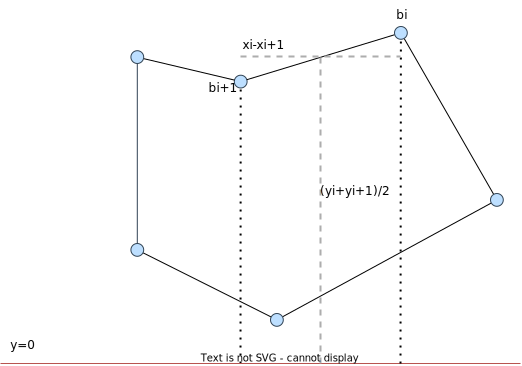
\includegraphics[width=.5\textwidth]{fig8.png}
  \caption{Vizualizace vzorce obsahu polygonu.}
\end{figure}
\end{multicols}{2}



\chapter{Rotace}

\begin{lstlisting}
./MP €\cmd{cube-example}€ 
\end{lstlisting}

\begin{figure}[H]
    \centering
    \includegraphics[width=1\textwidth]{fig10.png}
    \caption{3D rotace a projekce funguje v programu jako na obrázku. Pozorovatel (ohnisko) se pohybuje na sféře (převod souřadnic z jedné báze do druhé a rotace) a současně se dívá do středu souřadnic. 2D souřadnice se promítají na rovinu kolmou k spojnici střed-pozorovatel, která je posunuta dál od středu.}
    \label{fig:rotace_pozorovatel}
\end{figure}




\noindent
Otáčet bod vůči středu soustavy souřadné je jako nanášet ho na otočenou soustavu souřadnou, tedy násobit vektory udávájící osy $x$, $y$, atd. takové soustavy.
Tyto vektory mají délku 1. Lze zapsat takto:

$p_n = \begin{pmatrix}
X_1 & Y_1 \\
X_2 & Y_2
\end{pmatrix}\vec{p}$\\


\section{2D}

Otočené souřadnice můžeme vyjádřit takto:


$
X_1 = \cos(-\alpha) = \cos(\alpha)\\
X_2 = \sin(2\pi-\alpha) = -\sin(\alpha)\\
Y_1 = \cos(\pi/2 - \alpha) = \sin(\alpha)\\
Y_2 = \sin(\pi/2 - \alpha) = \cos(-\alpha) = \cos(\alpha)
$



$\begin{pmatrix}
\cos(\alpha) & \sin(\alpha)\\
-\sin(\alpha) & \cos(\alpha)
\end{pmatrix}\begin{pmatrix}x\\y\end{pmatrix}$



\section{3D}






Rotace bodu vůči ose Z ve směru hodinových ručiček:\\
$\begin{pmatrix}
\cos(\alpha) & \sin(\alpha) & 0\\
-\sin(\alpha) & \cos(\alpha) & 0\\
0 & 0 & 1
\end{pmatrix}\begin{pmatrix}x\\y\\z\end{pmatrix}$\\

\textbf{Rotace bodu vůči zvolené ose:}\cite{rotace}

Máme vstup osu $o$ a úhel $\alpha$. 

Mějme 2 soustavy souřadné $A$ a $B$ popsané jednotkovými vektory. Přitom $A$ je naše výchozí, na které vykreslujeme:

$\begin{pmatrix}
1 & 0 & 0\\
0 & 1 & 0\\
0 & 0 & 1
\end{pmatrix}$\\

Matice B má tvar:

$\begin{pmatrix}
a_x& b_x& o_x\\
a_y & b_y& o_y\\
a_z & b_z & o_z
\end{pmatrix}$\\

3. řádek $B$ tvoří souřadnice osy $o$, takže 3. souřadnice $p_b$ je právě vzhledem k $o$.

Čili je z následující rovnice zaručeno, že získáme přesně takový bod $p_b$, kde jeho 3. souřadnice je vzhledem k $o$. To potřebujeme, protože jsme zvolili matici
rotace podle osy Z (respektive 3. osy...), kterou chceme bod násobit. Takže tato souřadnice bodu v $B$ po rotaci bude stejná.

Z rovnice $p_a = p_b B$ vyjádříme tedy $p_b$ vynasobením $B^{-1}$: $p_b = p_a B^{-1}$\\ %!


Zbývající vektory $a$ a $b$ v $B$ musí být jednotkové a vzájemně kolmé. takový $a$ dostaneme třeba ignorováním $z$ a přehozením souřadnic následovně: $\vec{a} = \{-y, x, 0\}$, kde $x$ a $y$ jsou souřadnice $o$. $b$ je už jen vektorovým součinem $a$ a $b$.

To je tedy převod relativních souřadnic ze soustavy $A$ do soustavy $B$.

% Prakticky nesejde na určení výchozího směru rotace.



Rotace probíhá následovně:\\

Vstup: osa otáčení $o$, úhel $\alpha$

\begin{enumerate}[label=\arabic*, font=\bfseries] % nummbered list
	\item převedeme souřadnice z A do B
	\item zrotujeme (například přes matici 1.1, tj. vůči 3. ose)
	\item vykreslujeme v A, takže převedeme z B do A
\end{enumerate}

\section{Posunutí středu a osy otáčení}

Pro posunutý střed v 2D platí, že vektor $\vec{XS}$, kde $S$ je střed a $X$ bod, má fakticky souřadnice bodu $\vec{p}$. K výpočtu stačí potom přičíst $S$.\\

Stejně u posunuté osy v 3D, je takový vektor vlastně bod $p_a-S$.
V praxi, grafickém editoru, určujeme osu typicky dvěma body. Právě jeden z nich (třeba pro intuici první určený) je totiž tento střed $S$. Nakonec stačí opět přičíst $S$.


% TODO: krychle







\chapter{Generování tvarů} %a fraktály

\begin{lstlisting}[emph={:}]
./MP polygon|polygon-fill €\cmd{polygon-rnd:n:<int>}€
\end{lstlisting}

\begin{figure}[H]
  \centering
  \subfigure[Konkávní]{\includesvg[width=0.3\textwidth]{fig3}}
  \hfill
  \subfigure[Konvexní]{\includesvg[width=0.3\textwidth]{fig4}}
    \hfill
  \subfigure[Konkávní]{\includesvg[width=0.3\textwidth]{fig5}}
  \caption{Metody generování polygonu}
  \centering
\end{figure}
 
Generování náhodných polygonů není to samé co pouhé generování náhodných bodů - strany se mohou protínat či svírat úhel 180 stupňů, což bývá v praxi nežádoucí.
Metoda (a) je generování bodů na kružnici a následně vyběr náhodné pozice na pomyslné úsečce střed-bod.
První a poslední bod na kružnici zúžuje úhlový rozsah, v kterém další bod generujeme. Posledním bodem se pak stává generovaný bod a situace se opakuje. Hrany se nemohou protnout, protože se vždy nová hrana nachází celá ve zmíněné oblasti, kde žádný jiný bod neleží. Metoda může generovat konkávní polygony. Metoda (b) generuje na postupně procházených hranách trojúhelníku 1-2 náhodných bodů, v případné další iterace algoritmu se generuje nad výsledným tvarem atd. Následující iterací se dá generovat až dvojnásobný počet vrcholů tvaru z předchozí iterace. Výsledkem je konvexní polygon. Metoda (c) itereativně generuje body v určeném kvadrantu kartézských souřadnic, kde středem se následně stává generovaný bod. Díky tomu má generovaný bod ze všech nejmenší $x$ souřadnici. První bod má nejmenší $y$. Pro spojení prvního a posledního bodu se urči bod $[x,y]$, kde $x<minX$ a $y<minY$.


\pagebreak
Metoda (a):
\begin{enumerate}[label=\arabic*, font=\bfseries] % nummbered list
	\item generuj $n$ náhodných úhlů
	\item seřaď tyto úhly
	\item konečnou pozici bodu urči jako $random\_cislo*\vec{B-S}$
\end{enumerate}







 



%\begin{itemize}
%  \item 
%\end{itemize}



\chapter{Praktická část}

Výstupem programu je okno a text v terminálu, v kterém program běží.
Program je psán v jazyce C, tedy je před spuštěním kompilován následovně.
\begin{lstlisting}
git clone https://github.com/malirl/MP.git && cd resources/program; sudo make MP
\end{lstlisting}


\section{Syntax, ovládání, funkce}

Program běží ve dvou módech - první příkazový (PM), druhý vývojářský (VM).
Rozdíl mezi nimi je však jen v datech, které zpracovává.
Pro uvedení programu do PM je následující syntax:
\begin{lstlisting}
./MP nazev_obejktu parametr:hodnota parametr:hodnota ...
\end{lstlisting}
Pro uvedení programu do VM stačí čistě spustit:
\begin{lstlisting}
./MP
\end{lstlisting}
PM zpracovává jeden objekt/problém z příkazu, avšak VM jen volá soubor devtest.c, zdrojový kód, v kterým je možné nastavit příslušné vstupy a volat příslušné 
funkce.

\footnote{-.}

\begin{itemize}
  \item Parametrem může být objekt, jehož parametr:hodnota jsou odděleny čárkami.
  \item Pořadí parametrů může být libovolné.
  \item Nadbytečné parametry program ignoruje.
  \item Nevalidní vstup program vyrozumí a skončí.
  \item Posouvání šipkami, zoom kolečkem myši/touchpadem.
  \item Speciální objekt example slouží stejně jako VM, ale vstup podobjektů nastavuje přes pomocné funkce. Nakonec libovolný výstup podobjektů zabaluje do vlastního čili výstupu jednoho objektu.
\end{itemize}

\section{Požadavky, omezení}
 
Pro úspěšnou kompilaci je nutná instalace překladače gcc a multimediální knohovny SDL2 na Linuxu (X-window system/Wayland). Jiné platformy nebyly testovány  (stačí pouze přepsat Makefile).
 
 
\section{Struktura programu}
 
 SDL2 řeší v programu pouze vytvoření okna, vykreslení bodů na něm a zachytávání uživatelského vstupu.\cite{sdl2} Zpracování regulárních výrazů řeší knihovna (modul) tiny-regex.
\\
 
\textbf{Klíčové vlastnosti}

 \begin{itemize}
  \item Projekt se skládá z kontroleru, který validuje typ vstupu, nastavuje scénu, volá jednotlivá řešení v podsložkách jako /polygon ap.
  \item Dílčí řešení zapisuje do objektu body nebo podobjekty pro vykreslení. V případě, že je objekt součástí řešení a nevykresluje se, zapisuje do výstupu skládajícího se z dalších možných výstupů.
  \item Správně nastavený vstup objektu pro vykreslení je v syntaxi PM prostého/úplného tvaru vypsán před zpracováním.
  \item Vstup je předán main.c v podsložce dané úlohy, kde je případně upraven pro účely daného algoritmu.
\end{itemize}

\chapter{Závěr}
%\section{Stínění objektů v 3D}
%\section{Zoom}

\bibliography{text}
\bibliographystyle{plain}


\end{document}